% Created 2022-05-11 Wed 12:05
% Intended LaTeX compiler: pdflatex
\documentclass[t, unicode, 12pt, xdvipdfmx, aspectratio=169, bxjsarticle]{beamer}
\usepackage[utf8]{inputenc}
\usepackage[T1]{fontenc}
\usepackage{graphicx}
\usepackage{grffile}
\usepackage{longtable}
\usepackage{wrapfig}
\usepackage{rotating}
\usepackage[normalem]{ulem}
\usepackage{amsmath}
\usepackage{textcomp}
\usepackage{amssymb}
\usepackage{capt-of}
\usepackage{hyperref}
\usepackage[backend=bibtex, style=authoryear, maxcitenames=2]{biblatex}
\addbibresource{../resources/anthology.bib}
\addbibresource{../resources/my.bib}
\let\oldcite\cite
\renewcommand{\cite}[1]{{\scriptsize\reffont{(\oldcite{#1})}}}
\newcommand{\citet}[2][\footnotesize]{{\reffont#1\citeauthor*{#2} (\citeyear{#2})}}
\newcommand{\mycite}[1]{{\scriptsize\reffont({\citeauthor*{#1}, \citeyear{#1}})}}
\newcommand{\myfootcite}[1]{\footnote{\tiny\reffont\citetitle{#1}, \citeauthor*{#1}, \citeyear{#1}.}}
\usepackage{hyperref}
\usetheme{metropolis}
\setbeamertemplate{items}[default]
\setbeamertemplate{itemize item}{\small\raise0.5pt\hbox{$\blacksquare$}}
\setbeamertemplate{itemize subitem}{\footnotesize\raise1.5pt\hbox{$\bullet$}}
\setbeamertemplate{itemize subsubitem}{\scriptsize\raise1.5pt\hbox{$\blacktriangleright$}}
\setbeamertemplate{enumerate item}{\textbf{\arabic{enumi}.}}
\addtolength{\skip\footins}{6pc plus 10pt}
\usepackage{xltxtra}
\usepackage{booktabs}
\usepackage[absolute,overlay]{textpos}
\usepackage{pgfpages}
\usepackage{tikz}
\usepackage{tikz-dependency}
\usetikzlibrary{arrows.meta, matrix, positioning, fit, calc, backgrounds, shapes.callouts}
\usepackage{pgfgantt}
\usepackage{adjustbox}
\usepackage{array}
\usepackage[linguistics]{forest}
\newcommand{\highlightcap}[3][blue]{\tikz[baseline=(x.base)]{\node[rectangle,rounded corners,fill=#1!20](x){#2} node[below=0.5ex of x, color=#1]{#3};}}
\newcommand{\highlight}[2][blue]{\tikz[baseline=(x.base)]{\node[rectangle,rounded corners,fill=#1!20](x){#2};}}
\newcommand{\calloutbase}[2]{\tikz[remember picture, baseline=(#1.base)]{\node(#1) {#2};}}
\newcommand{\calloutpos}[2]{\tikz[remember picture, overlay]{\node[below=0cm of #1] {#2};}}
\newcommand{\calloutbelow}[3][blue]{\tikz[remember picture, overlay]{\node[rectangle callout, rounded corners, fill=#1!10, callout absolute pointer={(#2.south)}, below=of #2] {#3};}}
\usepackage{xcolor}
\definecolor{myalert}{HTML}{AD003D}
\definecolor{mDarkTeal}{HTML}{23373b}
\definecolor{mLightGreen}{HTML}{14B03D}
\usepackage{ulem}
\usefonttheme{professionalfonts}
\usepackage[T1]{fontenc}
\usepackage{fontspec}
\setsansfont[BoldFont={Fira Sans Bold}]{Fira Sans Book}
\newfontfamily\firasans{Fira Sans}
\newfontfamily\cica{Cica}
\newfontfamily\octicons{octicons}
\newfontfamily\materials{Material Icons}
\newfontfamily\faicons{FontAwesome}
\newfontfamily\reffont{Times New Roman}
\usepackage{amssymb}
\usepackage{mathfont}
\usepackage{bbm}
\renewcommand{\baselinestretch}{1.2}
\setbeamersize{text margin left=6mm}
\setbeamersize{text margin right=6mm}
\usetheme{default}
\author{\mbox{\lower2.0pt\hbox{\materials}}~ Hiroyuki Deguchi \\ \mbox{\lower2.0pt\hbox{\materials}}~ \texttt{deguchi.hiroyuki.db0@is.naist.jp} \\ \raise0.5pt\hbox{\octicons}~ \url{https://arxiv.org/abs/2204.05424} \\ \raise0.5pt\hbox{\octicons}~ \url{https://github.com/jungokasai/beam_with_patience}}
\date{\mbox{\lower2.0pt\hbox{\materials}}~ 2022/05/11 NAIST MT study group}
\title{Beam Decoding with Controlled Patience}
\subtitle{(Kasai et al., 2022)}
\institute{}
\hypersetup{
 pdfauthor={\mbox{\lower2.0pt\hbox{\materials}}~ Hiroyuki Deguchi \\ \mbox{\lower2.0pt\hbox{\materials}}~ \texttt{deguchi.hiroyuki.db0@is.naist.jp} \\ \raise0.5pt\hbox{\octicons}~ \url{https://arxiv.org/abs/2204.05424} \\ \raise0.5pt\hbox{\octicons}~ \url{https://github.com/jungokasai/beam_with_patience}},
 pdftitle={Beam Decoding with Controlled Patience},
 pdfkeywords={},
 pdfsubject={},
 pdfcreator={Emacs 27.1 (Org mode 9.3)}, 
 pdflang={English}}
\begin{document}

\maketitle

\begin{frame}[label={sec:orgd1eb8cc}]{Introduction}
\begin{block}{Beam search is widely used, but the implementation has variations.}
\begin{columns}
\begin{column}{0.5\columnwidth}
\begin{itemize}
\item \textbf{Vanilla}: TensorFlow Addons library
\item \textbf{\textit{first come, first served; FCFS}}: fairseq, Transformers
\begin{itemize}
\item This paper proposes a \textbf{\textit{patience factor}} on FCFS beam search.
\end{itemize}
\end{itemize}
\end{column}

\begin{column}{0.5\columnwidth}
\begin{center}
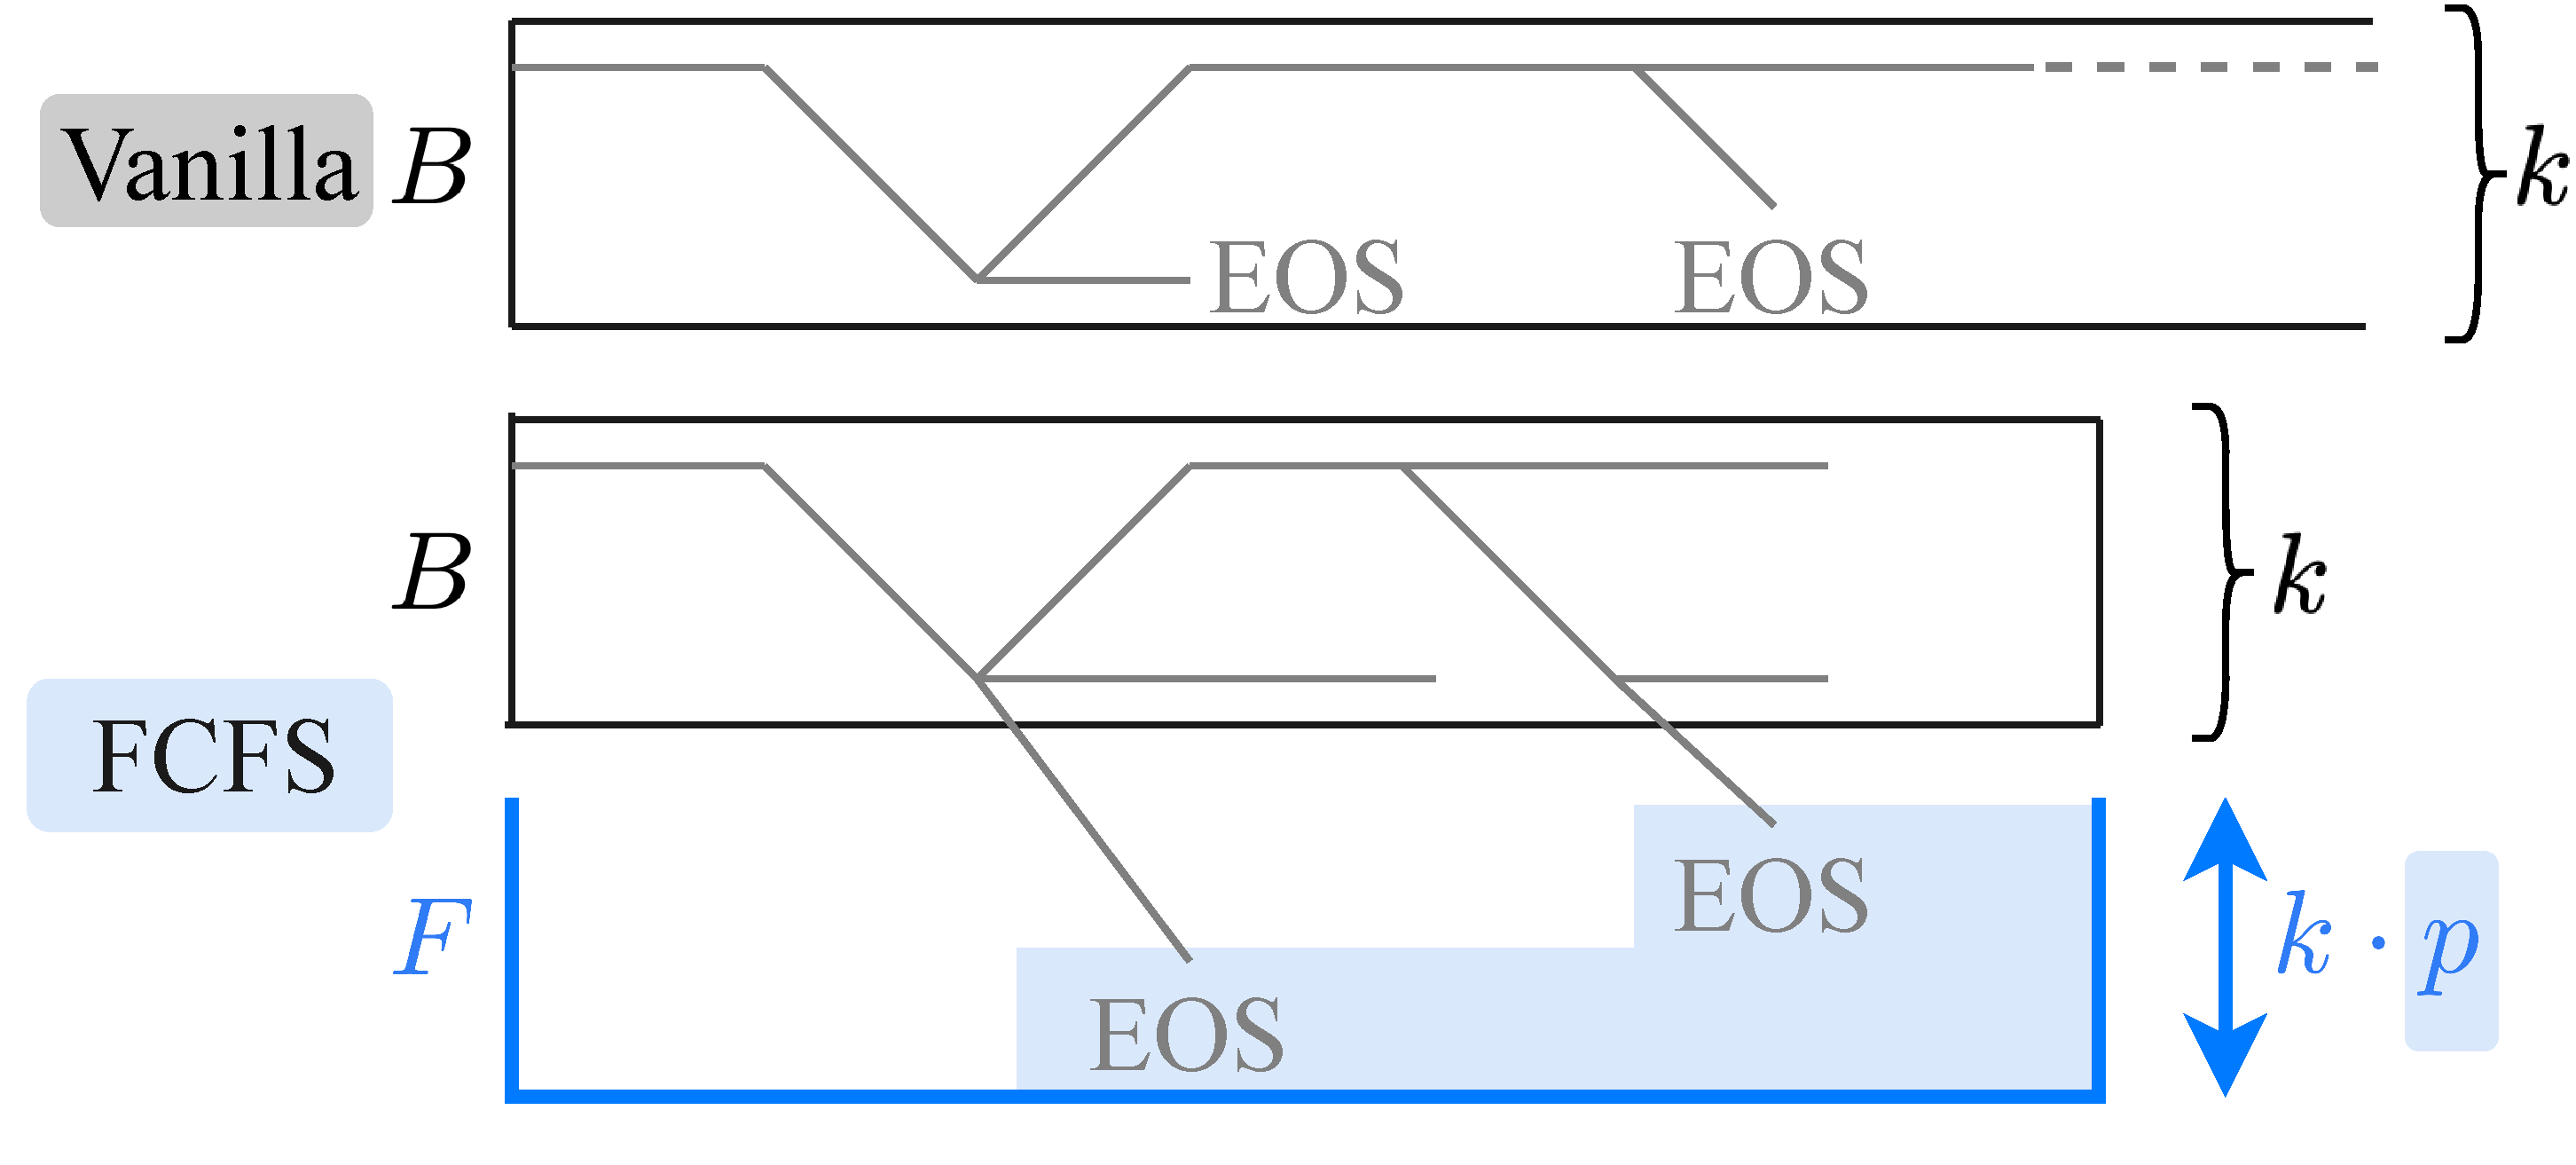
\includegraphics[width=1.0\linewidth]{./figure/contrast_fig.pdf}
\end{center}

\footnotesize \textbf{Vanilla vs. FCFS with patience factor $p$}: \\
\(k\) denotes the beam size. FCFS stores finished sentences in \(F\), but they stay in (and later may fall off from) beam \(B\) during vanilla decoding.
\end{column}
\end{columns}
\end{block}
\end{frame}

\begin{frame}[label={sec:org98134dc}]{Vanilla Beam Decoding}
\vspace{-0.2cm}
\begin{block}{The top-$k$ operation is applied over all sequences.}
\begin{columns}
\begin{column}{0.5\columnwidth}
\begin{itemize}
\item Find the top-\(k\) sequences, including both finished and unfinished sequences: \colorbox{red!15}{Line 5}
\item Decode until all top-\(k\) sequences are finished: \colorbox{green!25}{Line 13}
\begin{itemize}
\item It tends to result in deeper search.
\end{itemize}
\end{itemize}
\end{column}

\begin{column}{0.5\columnwidth}
\begin{center}
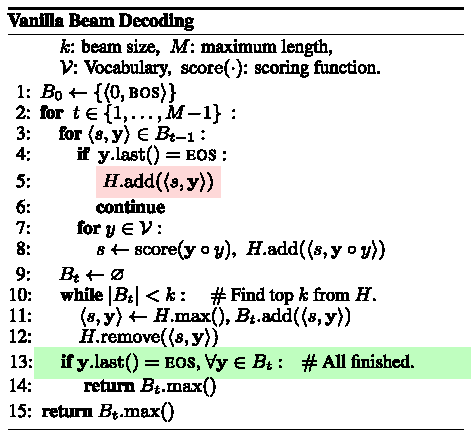
\includegraphics[width=0.95\linewidth]{./figure/vanilla.pdf}
\end{center}
\end{column}
\end{columns}
\end{block}
\end{frame}

\begin{frame}[label={sec:orgeeb1715}]{First Come, First Served (FCFS)}
\vspace{-0.2cm}
\begin{block}{The top-$k$ operation is applied over unfinished sequences.}
\begin{columns}
\begin{column}{0.5\columnwidth}
\begin{itemize}
\item Collect finished sequences in a \textit{first come, first served} manner and removes them from the beam: Line 11
\item FCFS has a wider breadth since it collects \(k\) unfinished sequences at every step regardless of how many sequences are finished with the EOS symbol.
\begin{itemize}
\item Terminate when a total of \(k\) finished sequences is found.
\end{itemize}
\end{itemize}
\end{column}

\begin{column}{0.5\columnwidth}
\vspace{-0.3cm}
\begin{center}
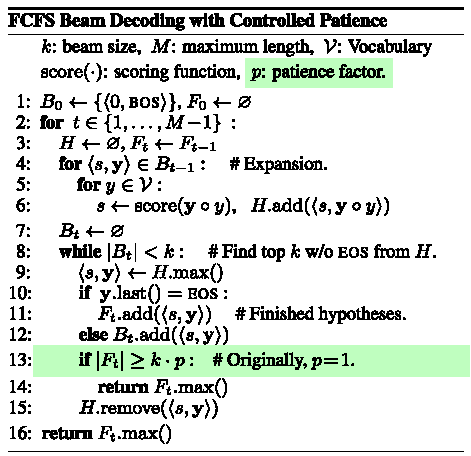
\includegraphics[width=0.95\linewidth]{./figure/FCFS.pdf}
\end{center}
\end{column}
\end{columns}
\end{block}
\end{frame}

\begin{frame}[label={sec:org7fc7405}]{Patience Factor for FCFS}
\vspace{-0.2cm}
\begin{block}{Separate the stopping criterion from the search breadth.}
\begin{columns}
\begin{column}{0.5\columnwidth}
\begin{itemize}
\item Beam size \(k\) in FCFS controls both the breadth and stopping criterion (i.e., depth) of search.
\item Proposed \textbf{patience factor} relaxes this assumption: \colorbox{green!25}{Line 13}
\begin{itemize}
\item It can be implemented by the one-line modification.
\end{itemize}
\end{itemize}
\end{column}

\begin{column}{0.5\columnwidth}
\vspace{-0.3cm}
\begin{center}
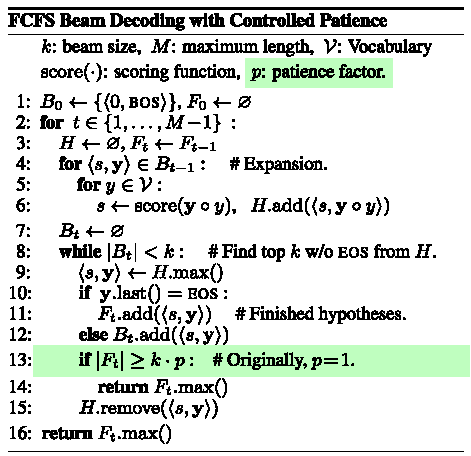
\includegraphics[width=0.95\linewidth]{./figure/FCFS.pdf}
\end{center}
\end{column}
\end{columns}
\end{block}
\end{frame}

\begin{frame}[label={sec:org2794efc}]{Main Results}
\vspace{-0.3cm}
\begin{itemize}
\item patience factor: \(p = 2\) for MT, \(p = 0.5\) for summarization
\item metric: COMET (XLM-RoBERTa) for MT, ROUGE for summarization
\end{itemize}
\vspace{-0.1cm}
\begin{center}
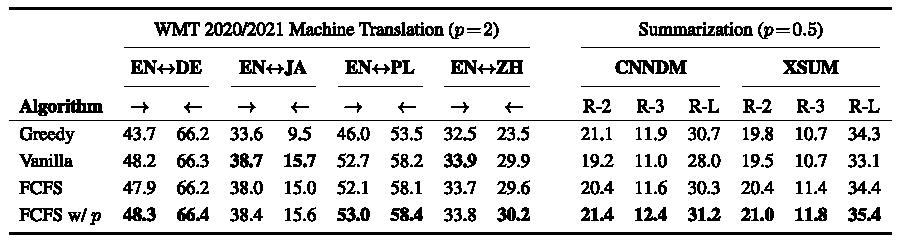
\includegraphics[width=0.9\linewidth]{./figure/main_results.pdf}
\end{center}
\vspace{-0.2cm}
\begin{itemize}
\item In summarization, \textit{vanilla} decoding performs worse than \textit{greedy}.
\begin{itemize}
\item It might be a reason why \textit{FCFS} is used instead of \textit{vanilla} in popular libraries.
\end{itemize}
\end{itemize}
\end{frame}

\begin{frame}[label={sec:orgb61dfc7}]{Evaluate Translation by BLEU}
\begin{itemize}
\item patience factor: \(p=2\)
\item metric: BLEU
\end{itemize}
\begin{center}
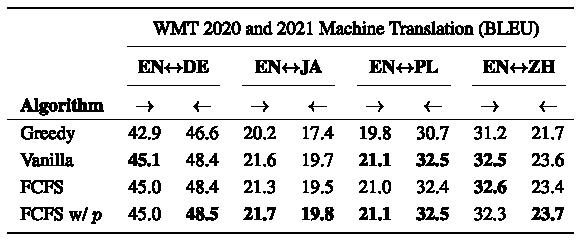
\includegraphics[width=0.75\linewidth]{./figure/mt_bleu.pdf}
\end{center}

\begin{itemize}
\item In many cases, \textit{FCFS w/$p$} slightly better than \textit{FCFS}.
\end{itemize}
\end{frame}

\begin{frame}[label={sec:org35498ef}]{Analysis: Effects of varying patience factors \(p\)}
\begin{center}
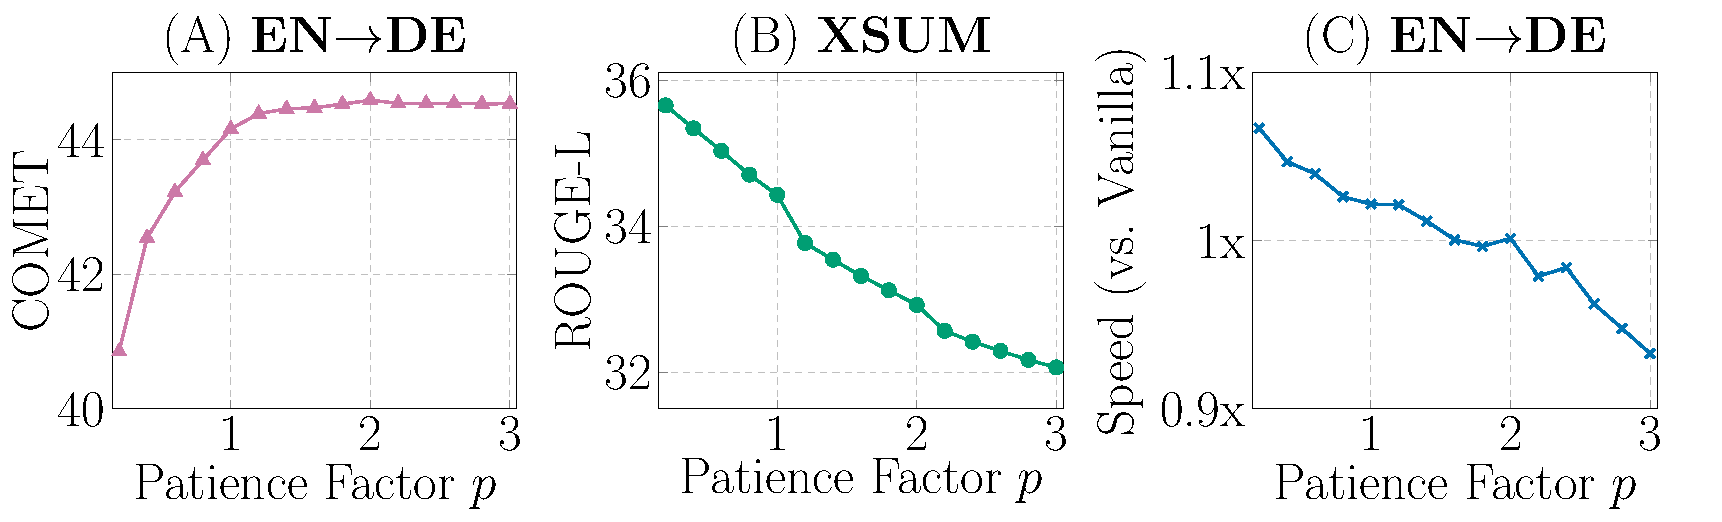
\includegraphics[width=0.8\linewidth]{./figure/varying_p.pdf}
\end{center}

\begin{itemize}
\item The translation performance improves with larger patience factors with diminishing gains.
\item Summarization benefits more from patience factors smaller than the original value of 1.
\begin{itemize}
\item The nature of the summarization task that aims to generate concise text.
\end{itemize}
\end{itemize}
\end{frame}

\begin{frame}[label={sec:org6c8ca4c}]{Analysis: Effects of controlled patience over varying beam sizes}
\begin{center}
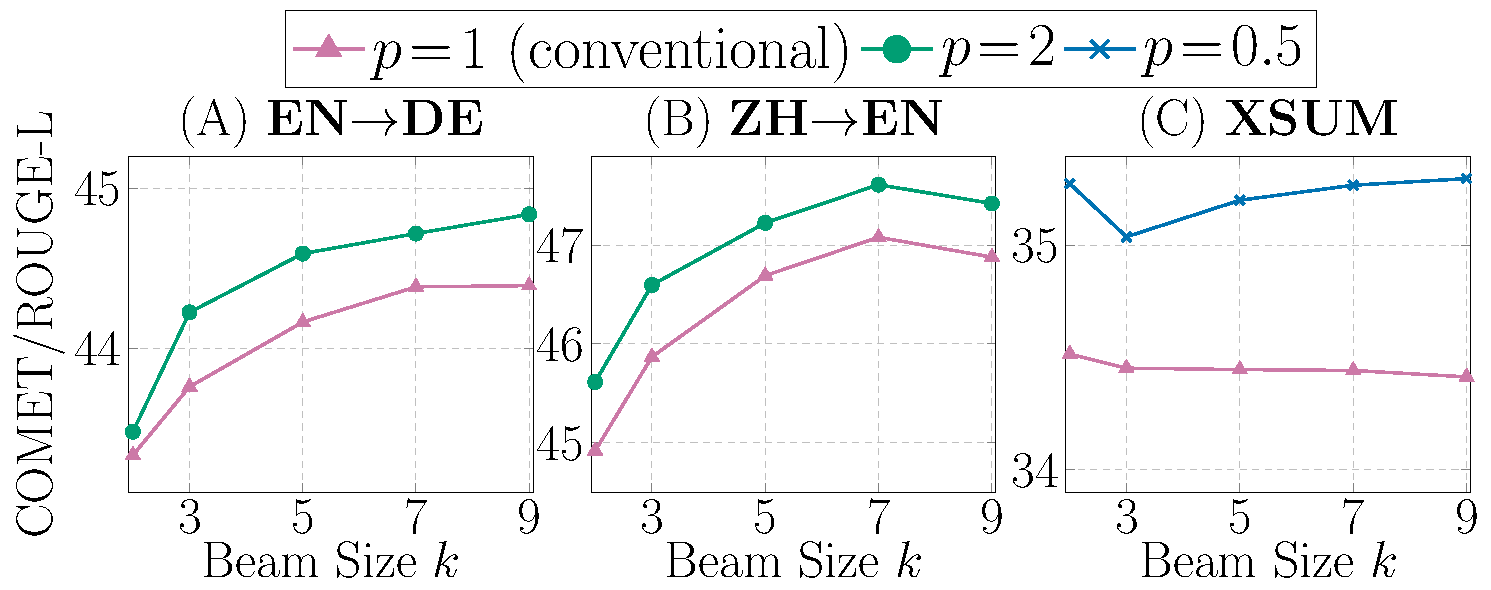
\includegraphics[width=0.65\linewidth]{./figure/varying_beam.pdf}
\end{center}

\vspace{-0.3cm}
\begin{itemize}
\item The amount of improvement changes, but the patience factor is generally beneficial.
\end{itemize}
\end{frame}

\begin{frame}[label={sec:orgeaa4f50}]{\normalsize Analysis: Effects of controlled patience over varying length penalty}
\begin{center}
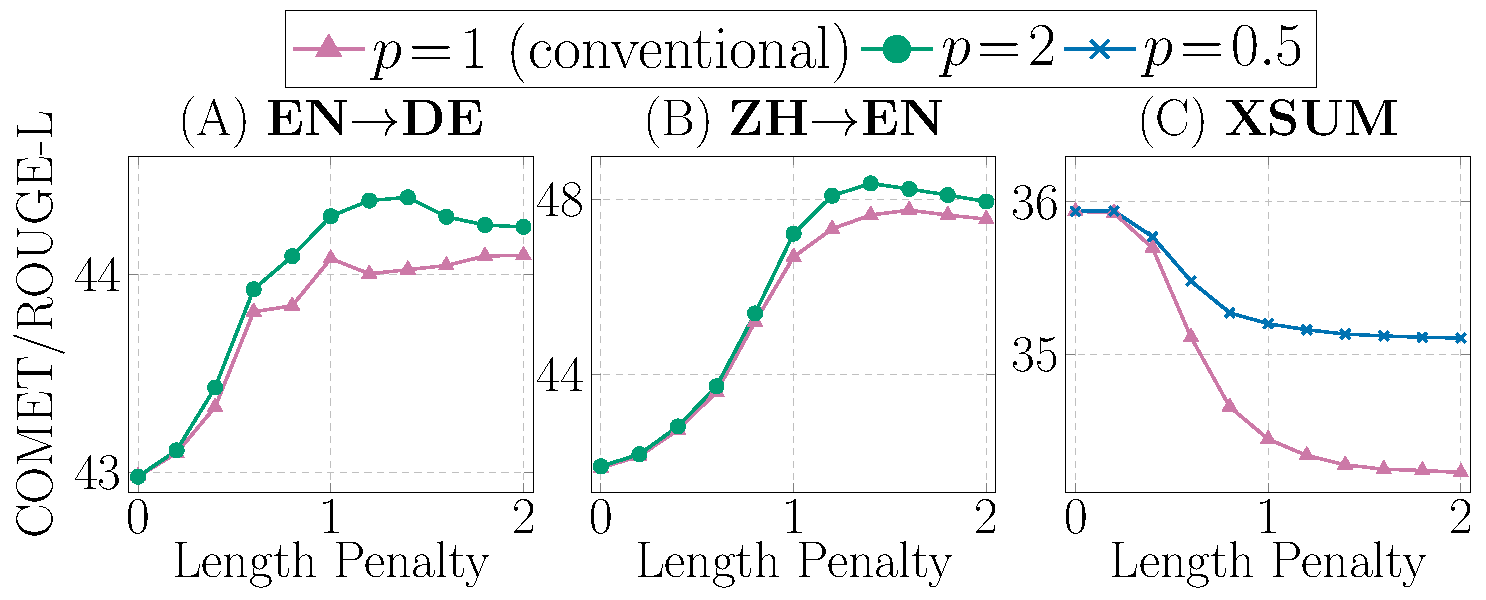
\includegraphics[width=0.65\linewidth]{./figure/varying_lenpen.pdf}
\end{center}

\vspace{-0.3cm}
\begin{itemize}
\item The amount of improvement changes, but the patience factor is generally beneficial.
\end{itemize}
\end{frame}

\begin{frame}[label={sec:org7b1d9a5}]{[BTW] Length Penalty}
\begin{itemize}
\item Length-normalized log probability:
\begin{equation*}
    \frac{\log (P(Y|X))}{\mathrm{lenpen}(Y)}
\end{equation*}

\begin{itemize}
\item Google NMT: \(\mathrm{lenpen}(Y) = \left(\frac{5 + |Y|}{5 + 1}\right)^\alpha\), \(\alpha = 0.6\)
\item Fairseq: \(\mathrm{lenpen}(Y) = |Y|^\alpha\), \(\alpha = 1.0\)
\begin{itemize}
\item This paper uses the fairseq version's length penalty.
\end{itemize}
\end{itemize}
\end{itemize}
\end{frame}


\begin{frame}[label={sec:org1c8697a}]{Related Work}
\begin{block}{Stopping Criterion for Beam Decoding}
\begin{itemize}
\item Optimal Beam Search (Huang et al., EMNLP 2017)\myfootcite{huang-etal-2017-finish}
\begin{itemize}
\item They propose a method to optimally finish beam search.
\item Modify the beam decoding procedure
\end{itemize}
\end{itemize}
\end{block}

\begin{block}{Breadth of Beam Decoding}
\begin{itemize}
\item Analyzing effects of the search breadth (Ott et al., ICML 2018)\myfootcite{ott-etal-2018-analyzing}
\end{itemize}
\end{block}
\end{frame}

\begin{frame}[label={sec:orgeebf6a0}]{Conclusion}
\begin{columns}
\begin{column}{0.6\columnwidth}
\begin{itemize}
\item This paper named two major beam search implementation, vanilla and FCFS.
\item This paper proposed \textbf{patience factor} for FCFS, controls the stopping criterion.
\item Experiments shows that the proposed FCFS w/patience gains better translation/summarization performance than FCFS.
\end{itemize}
\end{column}

\begin{column}{0.4\columnwidth}
\begin{center}
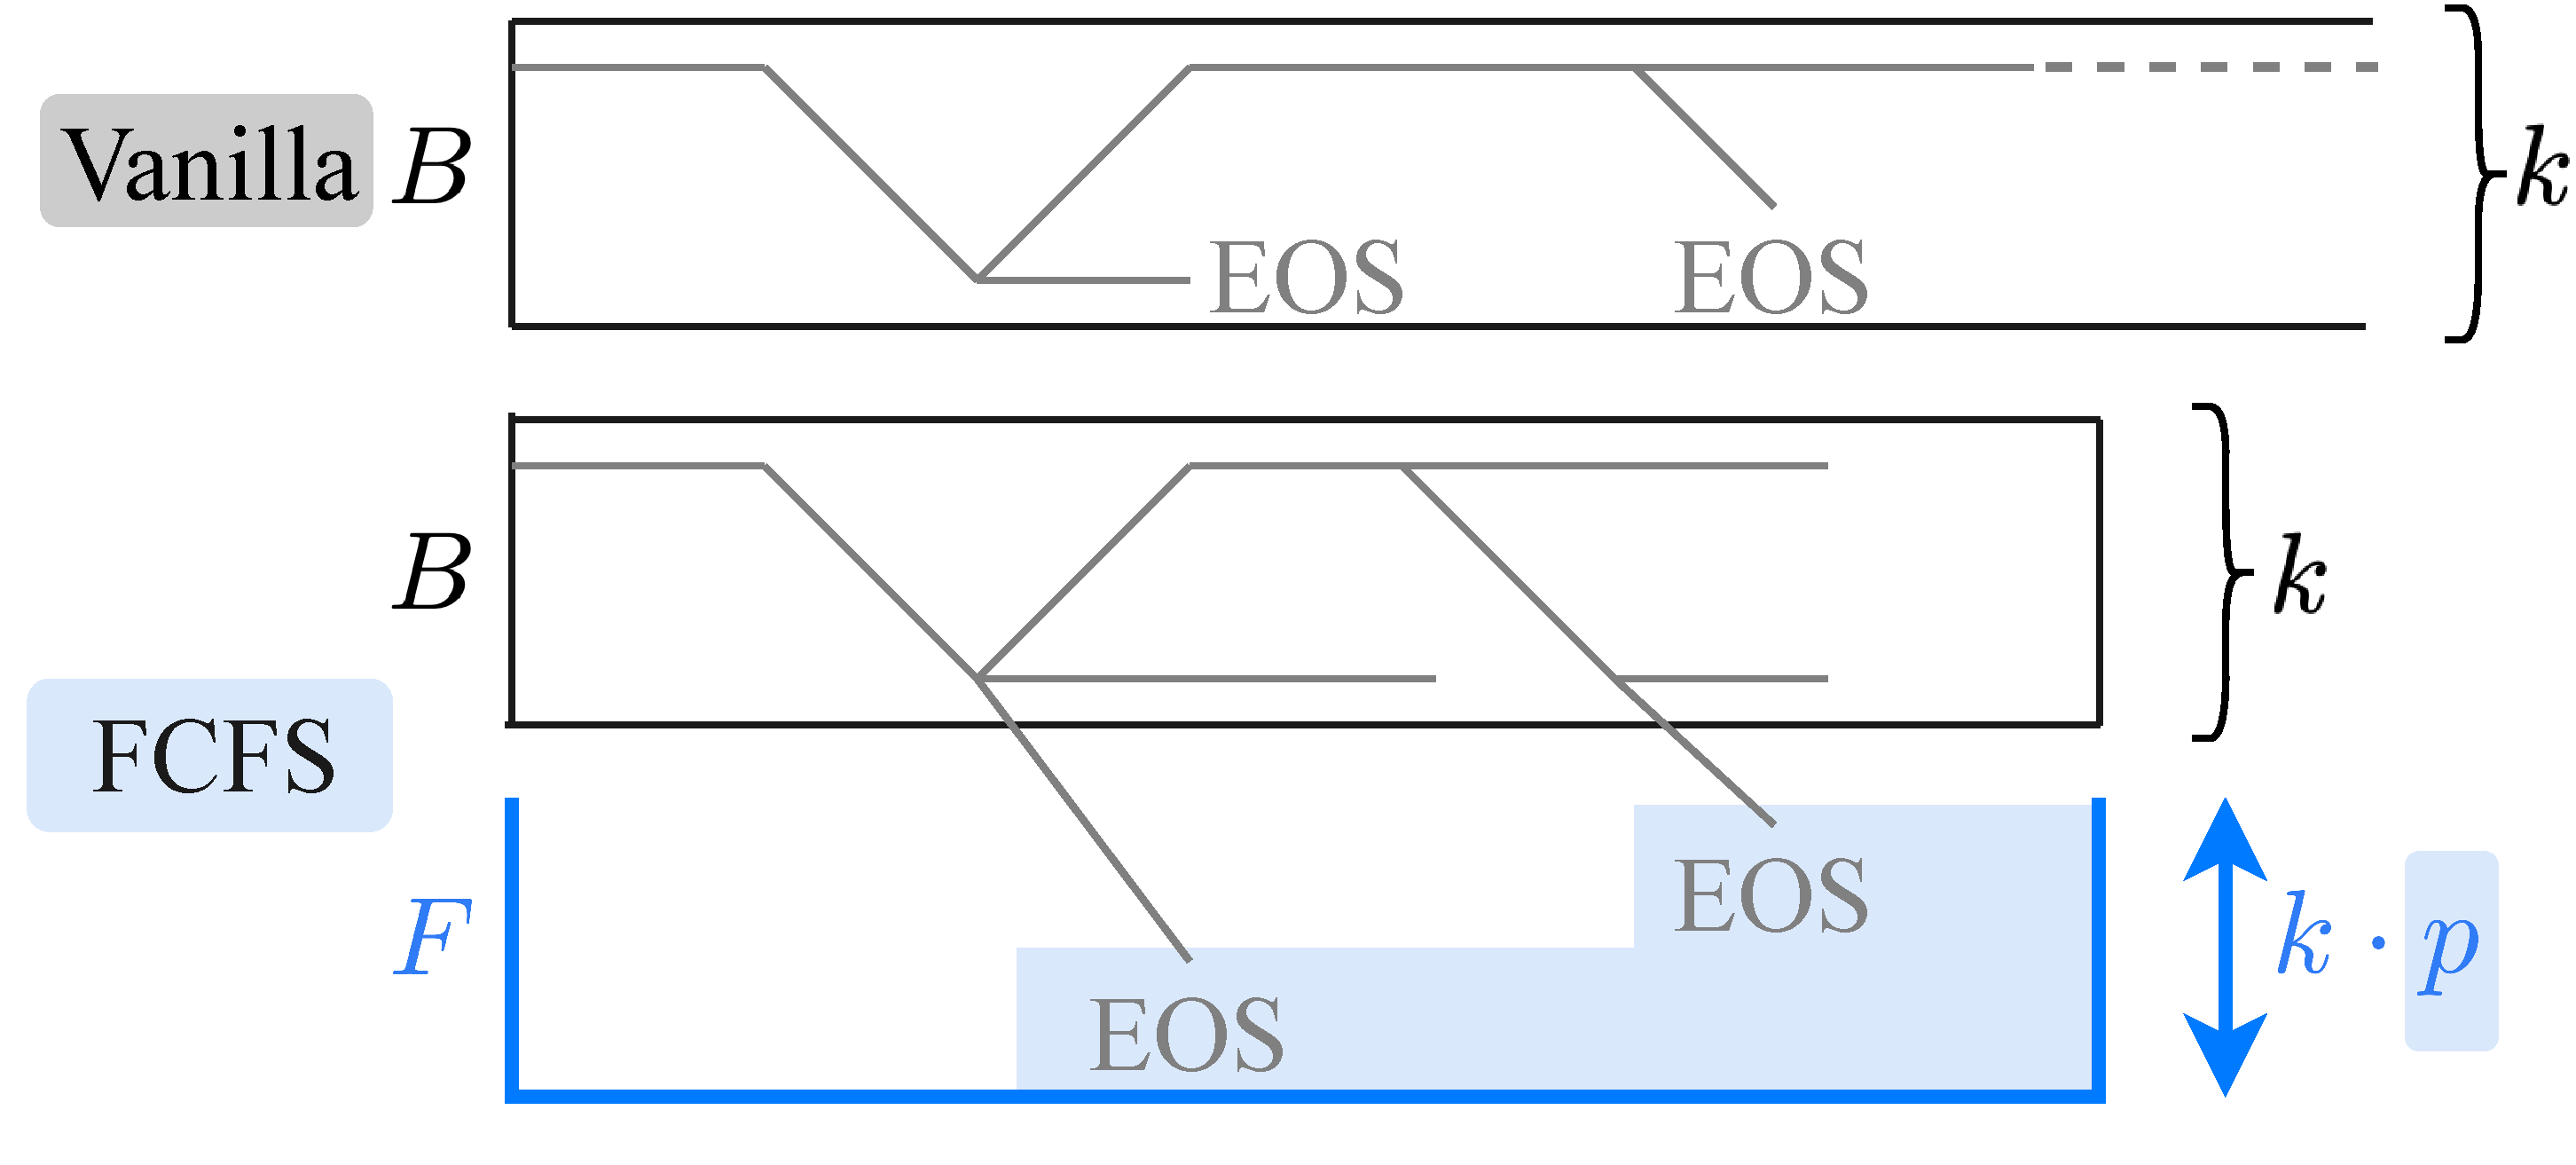
\includegraphics[width=1.0\linewidth]{./figure/contrast_fig.pdf}
\end{center}
\end{column}
\end{columns}
\end{frame}
\end{document}